\section{Power}
\subsection{Power supply}
The card can operate connested to SAYMA AMC card. When the card is inserted to the SAYMA AMC,  the power is applied from RTM connector -J2, +12V (4 power lines) and +3.3\_MP(1 line). Both voltages can be controlled by SAYMA AMC.
+12 is converted to lower voltages and negative voltages, simplified power map is in figure \ref{powermap}. There are few types of power distributors, fixed LDOs, Buck converters and Exar chip - quad channel digital Pulse Width Modulated (PWM) step down (buck) controller. Exar allows for adjust power parameters and for set particular power oorder. Exar firmware monitors current and responds if its too high.  Additionaly all LDOs have connected PowerGood outputs so it is possible to read the proper state of all power busses. 

\todo[inline]{TBD voltage noise}



%Maximum board(AMC+RTM module) power consumption estimate to 3A @ 12V.\\
%
%	\textit{\textbf{Note:} Please note that power consumption mostly depends from FPGA configuration. \\}

\begin{itemize}
 

\item Input voltage range: 10.8-13.2 [V]\\
\item The board needs active cooling. Approx. 20CFM in 20 C air.\\

\end{itemize}

Exar chips are configured via EXAR\_I2C bus (I2CMUX7) or directly by connecting to W1 
%(call-out 28) 
header. For proper configuration \textbf{Exar Power Architect} in version \textbf{5.2-r1} is needed.
% Configuration files can be found at github in folder \href{https://github.com/m-labs/sinara/tree/master/EXAR\_config}{m-labs/sinara/Exar\_config}\\

\noindent
\textbf{Exar Power Archtect 5.2-r1:}
\href{https://www.exar.com/content/document.ashx?id=21632}{https://www.exar.com/content/document.ashx?id=21632}\\
\textbf{Configuration files:}
\href{https://github.com/m-labs/sinara/tree/master/EXAR\_config}{https://github.com/m-labs/sinara/tree/master/EXAR\_config}\\
\textbf{Datasheet:}\href{https://www.exar.com/ds/xr77129_1a_120514.pdf}{https://www.exar.com/ds/xr77129\_1a\_120514.pdf}\\
\textbf{Quick Start Guide:} \href{https://www.exar.com/files/powerxr/PA5-QSG_110_010614.pdf}{https://www.exar.com/files/powerxr/PA5-QSG\_110\_010614.pdf}\\


Actual voltages and current consumption, temperature can be found in Chip Dashboard. There is also oportunity to adjust settings.

\begin{figure}[htbp!]
	\centering
	\includegraphics[scale=0.6]{img/exarprog.png}\\
	\caption{Chip Dashboard} 
\end{figure}

\clearpage
\subsection{Power configuration} 

\subsubsection{Power map}


	\begin{figure}[htbp!]
		\centering
		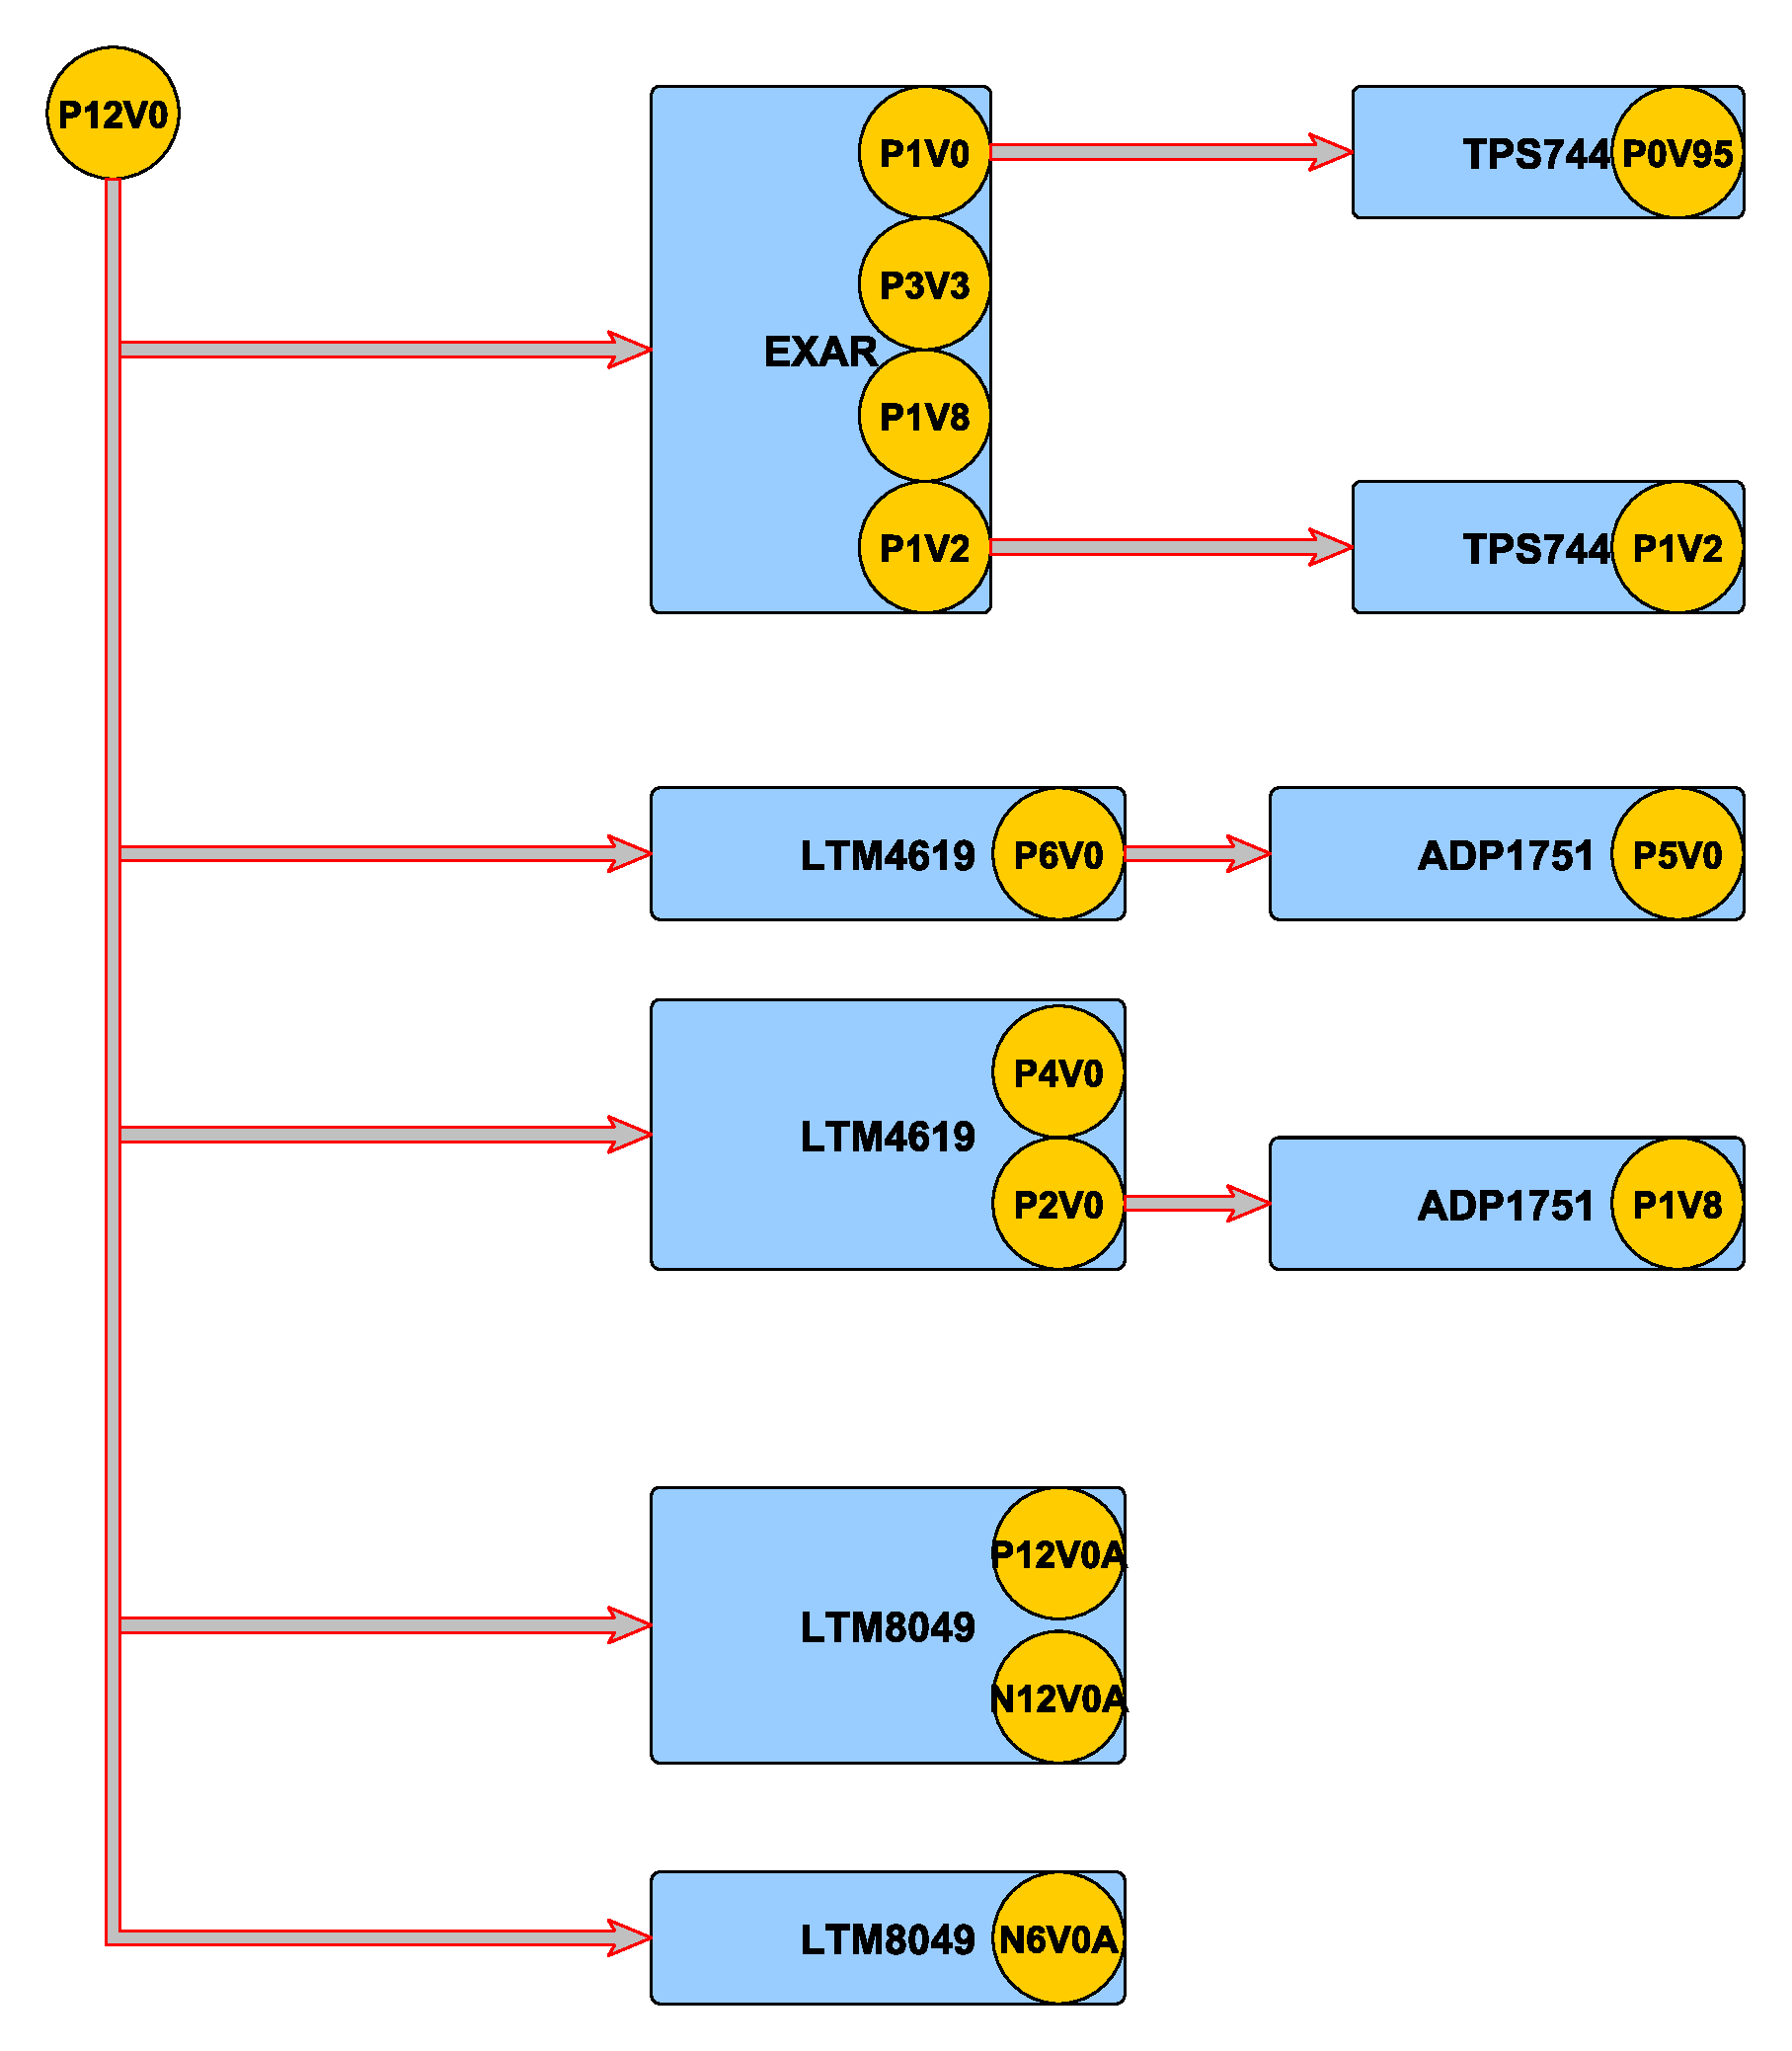
\includegraphics[scale=0.3]{img/pwr.eps}\\
		\caption{Power map} \label{powermap}
	\end{figure}
	

\begin{longtable}{|c|c|c|} \hline
\multicolumn{3}{|c|}{voltages and currents}	\\ \hline
P1V0 & 1.0V & 4A \\ \hline
P1V2 & 1.2V & 2A\\ \hline
P1V8 & 1.8V & 2A\\ \hline
P2V0 & 2.0V & 4A\\ \hline
P3V3 & 3.3V & 4A\\ \hline
P4V0 & 4.0V & 4A\\ \hline
P6V0 & 6.0V & 8A\\ \hline
P12V0A & 12.0V & 1A \\ \hline
N6V0A & -6.0V & 4A\\ \hline
N12V0A & -12.0V & 1A \\ \hline

\end{longtable}
	
\subsubsection{Exar parameters}

Exar chip(XR77129) has 4 configurable outputs with configirable current limits. Each channel can be confugured individually. It is possible to set voltage, current limit and power sequencing. In Figure \ref{exar1} we can see that main power supply is 12V, Under Voltage Lockout(UVLO) is set to 6V, so below this value chip will shutdown all channels. When the temperature rise under Over Temperature Protection (OTP) 105 degrees, the chip will generate warning event and restart. \\
All 4 channells can be grouped together and will start-up and shut-down in an user defined sequwnce. Selecting none means channels will not be assigned to any group and therefore, will be controlled independently. Group 0 is controlled by ENABLE or EXAR\_I2C command. Group 1 can be controlled by GPIO or by EXAR\_I2C command. By selecting 'Wait PGOOD' next channel will not power up untill current channel reaches the target level. Delay is an additional delay time which postpone after power up one and another channel in group.\\
In on-going Exar configuration - Figure \ref{exar2}, power sequencing looks like this: After Enable - EN\_DC\_DC, P1V0 start-up, after it reaches proper value, Exar turn ramp up another channel in this group - P3V3. In the same order are ramp up next two channels in this group.



	\begin{figure}[htbp!]
		\centering
		\includegraphics[scale=0.5]{img/exar1.png}\\
		\caption{Exar configuration} \label{exar1}
	\end{figure}
\clearpage	
	\begin{figure}[htbp!]
		\centering
		\includegraphics[scale=0.5]{img/exar2.png}\\
		\caption{Exar power on delays} \label{exar2}
	\end{figure}	
	



%\subsubsection{Exar configuration}
%Exar chips are configured via I2C bus (MUX Port 5) or directly by connecting to W1 (call-out 28) header. For proper configuration \textbf{Exar Power Architect} in version \textbf{5.2-r1} is needed.
%% Configuration files can be found at github in folder \href{https://github.com/m-labs/sinara/tree/master/EXAR\_config}{m-labs/sinara/Exar\_config}\\
%
%\noindent
%\textbf{Exar Power Archtect 5.2-r1:}
%\href{https://www.exar.com/content/document.ashx?id=21632}{https://www.exar.com/content/document.ashx?id=21632}\\
%\textbf{Configuration files:}
%\href{https://github.com/m-labs/sinara/tree/master/EXAR\_config}{https://github.com/m-labs/sinara/tree/master/EXAR\_config}\\
%\textbf{Datasheet:}\href{https://www.exar.com/ds/xr77129_1a_120514.pdf}{https://www.exar.com/ds/xr77129\_1a\_120514.pdf}\\
%\textbf{Quick Start Guide:} \href{https://www.exar.com/files/powerxr/PA5-QSG_110_010614.pdf}{https://www.exar.com/files/powerxr/PA5-QSG\_110\_010614.pdf}\\
%
%
%Actual voltages and current consumption, temperature can be found in Chip Dashboard. There is also oportunity to adjust settings.
%
%	\begin{figure}[htbp!]
%		\centering
%		\includegraphics[scale=0.6]{img/exarprog.png}\\
%		\caption{Chip Dashboard} 
%	\end{figure}
%
\subsection{Maximum power draw for each Mezzaninne}

\begin{longtable}{|c|c|} \hline
	Power rail[V] & Current [mA]\\ \hline
	+12 & 200 \\ \hline
	-12 & 50 \\ \hline
	+6 & 1500 \\ \hline
	-6 & 100 \\ \hline
	+3.3 & 1000 \\ \hline
	
\end{longtable}	
